% !TEX root = ../../main.tex

\subsection{Vapour adsorption}

The effects of shaping with \(\rho\)-alumina are 
so far more subtle than the changes encountered when using 
PVA, as shown in the corresponding 
study~\cite{chanutObservingEffectsShaping2016}.
The influence of the binder on hydrophobic character of the
material may be of interest for tuning the properties of the 
beads. Adsorption of water and methanol vapour can serve as 
a probe for small changes is surface properties.
To this end, the same PVA samples which were 
studied in the previous study were studied alongside 
the MRA-shaped MOF.

Due to its surface charges, alumina is a 
hydrophilic substance, with a contact 
angle of \SI{10}{\degree}. It is expected that its 
addition will therefore increase the affinity 
of the resulting pellet towards water. On the other hand,
the PVA binder is more hydrophilic, with a water contact
angle of \SI{51}{\degree}. The medium affinity for water
is due to the surface hydroxyl functionalizations, which
can lead to hydrogen bonding.

Two indicators may highlight 
changes in material hydrophilicity: adsorption in the 
low relative pressure region (\(p/p^0 < 0.3\)) and 
condensation steps in the isotherm. The adsorption at low
pressures is representative of the first interactions with the 
surface, as explained in the previous sections. The pressure 
at which condensation occurs in the pores of the material, or 
where a sharp isotherm increase is seen depends on the 
size of the pore, but also on the pore environment and 
guest-guest interactions.

The measured isotherms on water and methanol can be found
in \autoref{fgr:shaping:wateradsorption} 
and \autoref{fgr:shaping:methanoladsorption} respectively.
The isotherms measured on the original powder materials 
show the normal adsorption behaviour which can then be 
compared with the MRA and PVA shaped samples. 

On UiO-66(Zr), the water isotherm shows a slow uptake at the 
start, corresponding to a hydrophobic material and then shows 
a small step at \(p/p^0 = 0.3\). Complete pore filling happens 
at \(p/p^0 = 0.8\).

Water isotherms on MIL-100(Fe) show a more hydrophilic environment,
with a higher initial uptake, and two condensation steps at 
\(p/p^0 = 0.3\) and \(p/p^0 = 0.5\). There is pronounced 
hysteresis on the desorption branch.
The methanol adsorption isotherms also show a two step adsorption
isotherm, but without any hysteresis present. The shaped samples 
also show a lower 

It can be therefore concluded that overall, the addition of either 
binder has not influenced the behaviour towards water or 
methanol for the materials studied. The full water adsorption isotherms
can be found in \autoref{fgr:shaping:wateradsorption}.

\begin{figure}[p!]
    \centering

    \begin{subfigure}{\linewidth}
        \centering
        \parbox{0.1\linewidth}{\caption{}\label{fgr:shaping:wateruio66}}%
        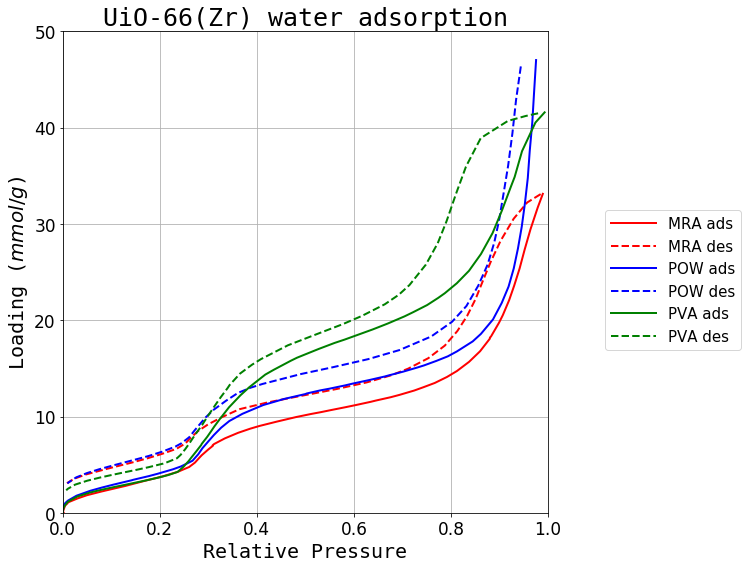
\includegraphics[width=0.4\textwidth]{water/UiO-66(Zr)-water}%
        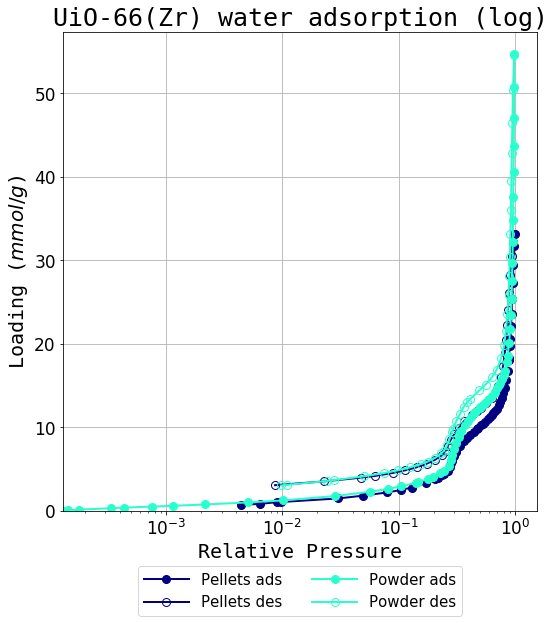
\includegraphics[width=0.4\textwidth]{water/UiO-66(Zr)-water-log}%
    \end{subfigure}

    \begin{subfigure}{\linewidth}
        \centering
        \parbox{0.1\linewidth}{\caption{}\label{fgr:shaping:watermil100}}%
        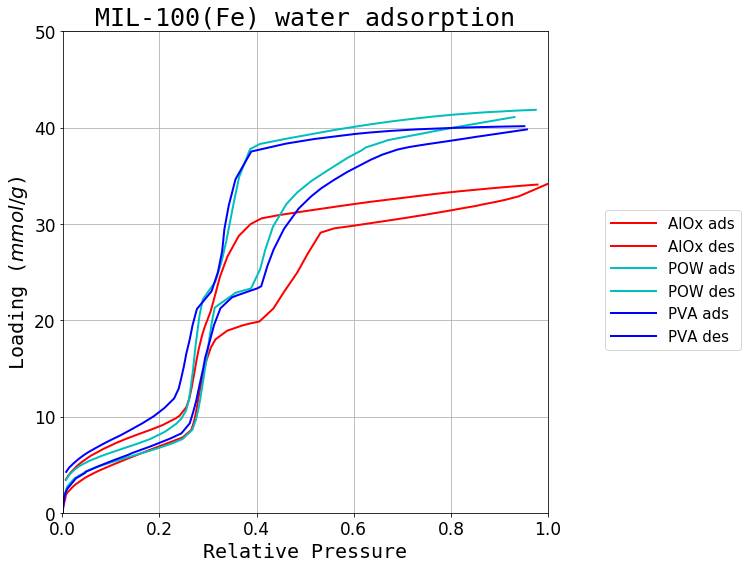
\includegraphics[width=0.4\textwidth]{water/MIL-100(Fe)-water}%
        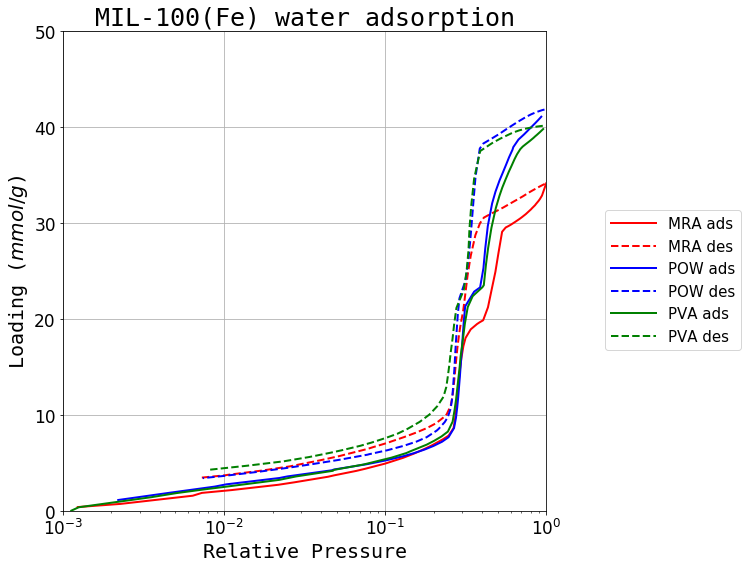
\includegraphics[width=0.4\textwidth]{water/MIL-100(Fe)-water-log}%
    \end{subfigure}

    \begin{subfigure}{\linewidth}
        \centering
        \parbox{0.1\linewidth}{\caption{}\label{fgr:shaping:watermil127}}%
        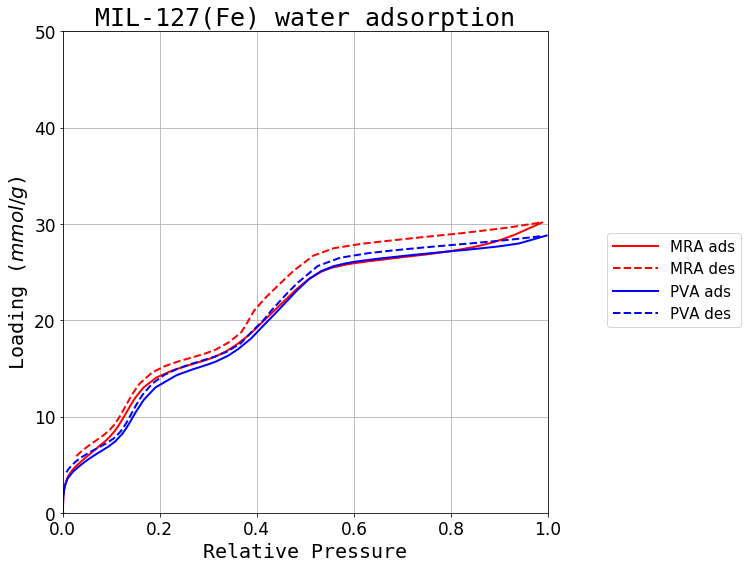
\includegraphics[width=0.4\textwidth]{water/MIL-127(Fe)-water}%
        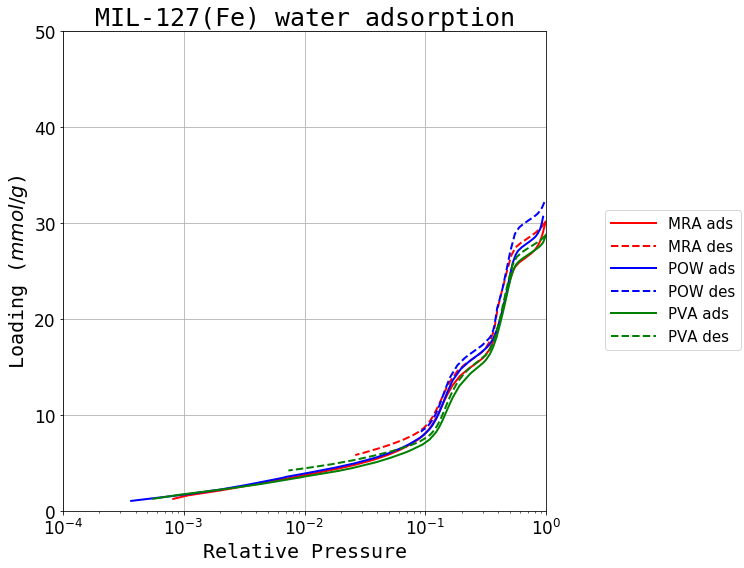
\includegraphics[width=0.4\textwidth]{water/MIL-127(Fe)-water-log}%
    \end{subfigure}
    
    \caption{Water adsorption isotherms (a) UiO-66(Zr), 
    (b) MIL-100(Fe) and (c) MIL-127(Fe). The powder samples are in light
    blue, while the \(\rho\)-alumina and poly-vinyl alcohol samples are in red
    and dark blue respectively. Logarithmic graphs of the isotherms are
    on the right for clarity of the low
    pressure region.}%
    \label{fgr:shaping:wateradsorption}
\end{figure}


\begin{figure}[p!]
    \centering

    \begin{subfigure}{\linewidth}
        \centering
        \parbox{0.1\linewidth}{\caption{}\label{fgr:shaping:methanoluio66}}%
        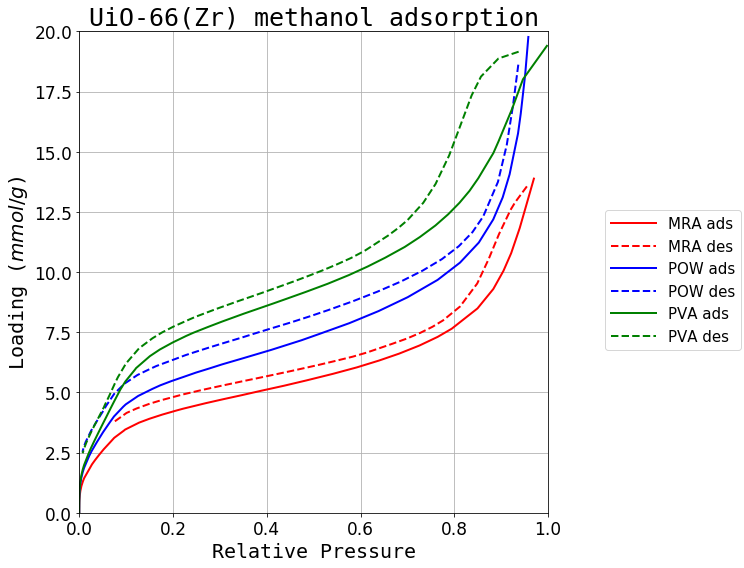
\includegraphics[width=0.4\textwidth]{methanol/UiO-66(Zr)-methanol}%
        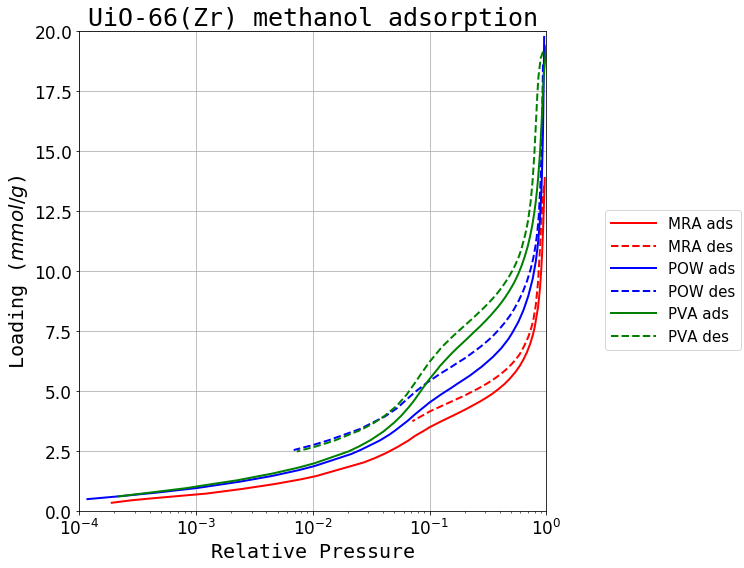
\includegraphics[width=0.4\textwidth]{methanol/UiO-66(Zr)-methanol-log}%
    \end{subfigure}

    \begin{subfigure}{\linewidth}
        \centering
        \parbox{0.1\linewidth}{\caption{}\label{fgr:shaping:methanolmil100}}%
        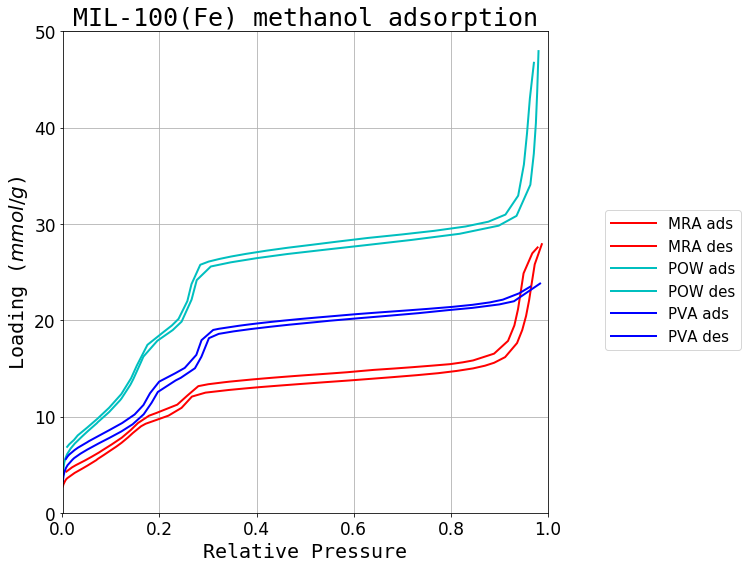
\includegraphics[width=0.4\textwidth]{methanol/MIL-100(Fe)-methanol}%
        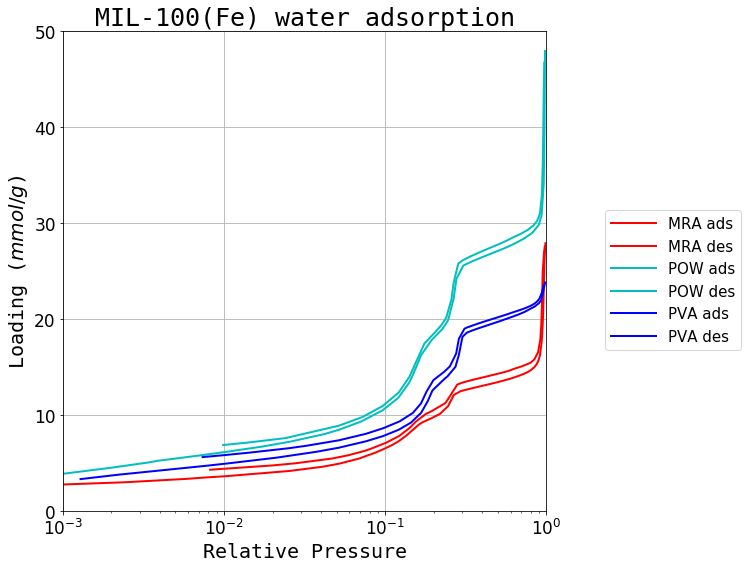
\includegraphics[width=0.4\textwidth]{methanol/MIL-100(Fe)-methanol-log}%
    \end{subfigure}

    \begin{subfigure}{\linewidth}
        \centering
        \parbox{0.1\linewidth}{\caption{}\label{fgr:shaping:methanolmil127}}%
        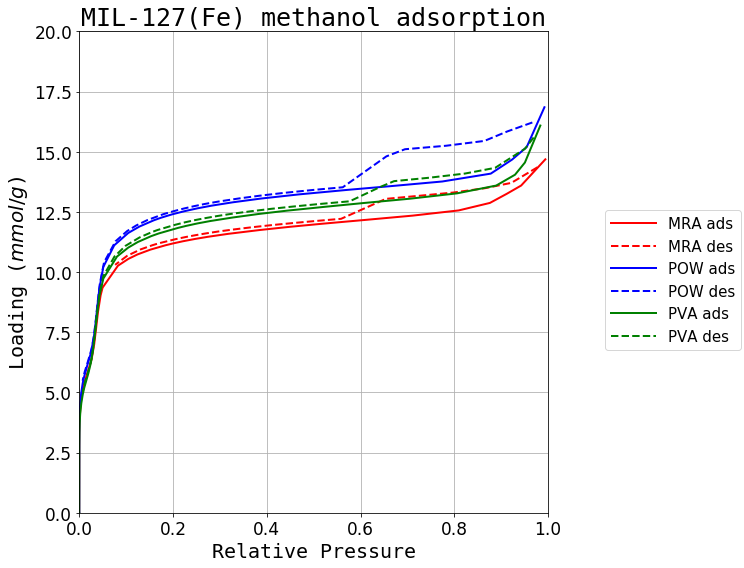
\includegraphics[width=0.4\textwidth]{methanol/MIL-127(Fe)-methanol}%
        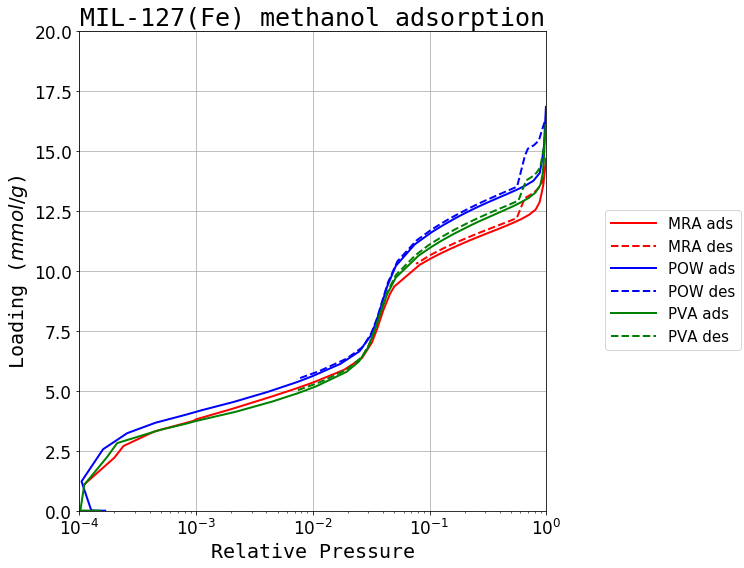
\includegraphics[width=0.4\textwidth]{methanol/MIL-127(Fe)-methanol-log}%
    \end{subfigure}
    
    \caption{Methanol adsorption isotherms (a) UiO-66(Zr), 
    (b) MIL-100(Fe) and (c) MIL-127(Fe). The powder samples are in light
    blue, while the \(\rho\)-alumina and poly-vinyl alcohol samples 
    are in red and dark blue respectively. Logarithmic graphs of
    the isotherms are
    on the right for clarity of the low
    pressure region.}%
    \label{fgr:shaping:methanoladsorption}
\end{figure}